\chapter{Anexos}\label{sec:Anexos}

\section{Diagrama de Bloques del sistema completo}

\begin{figure*}[h!]
\centering
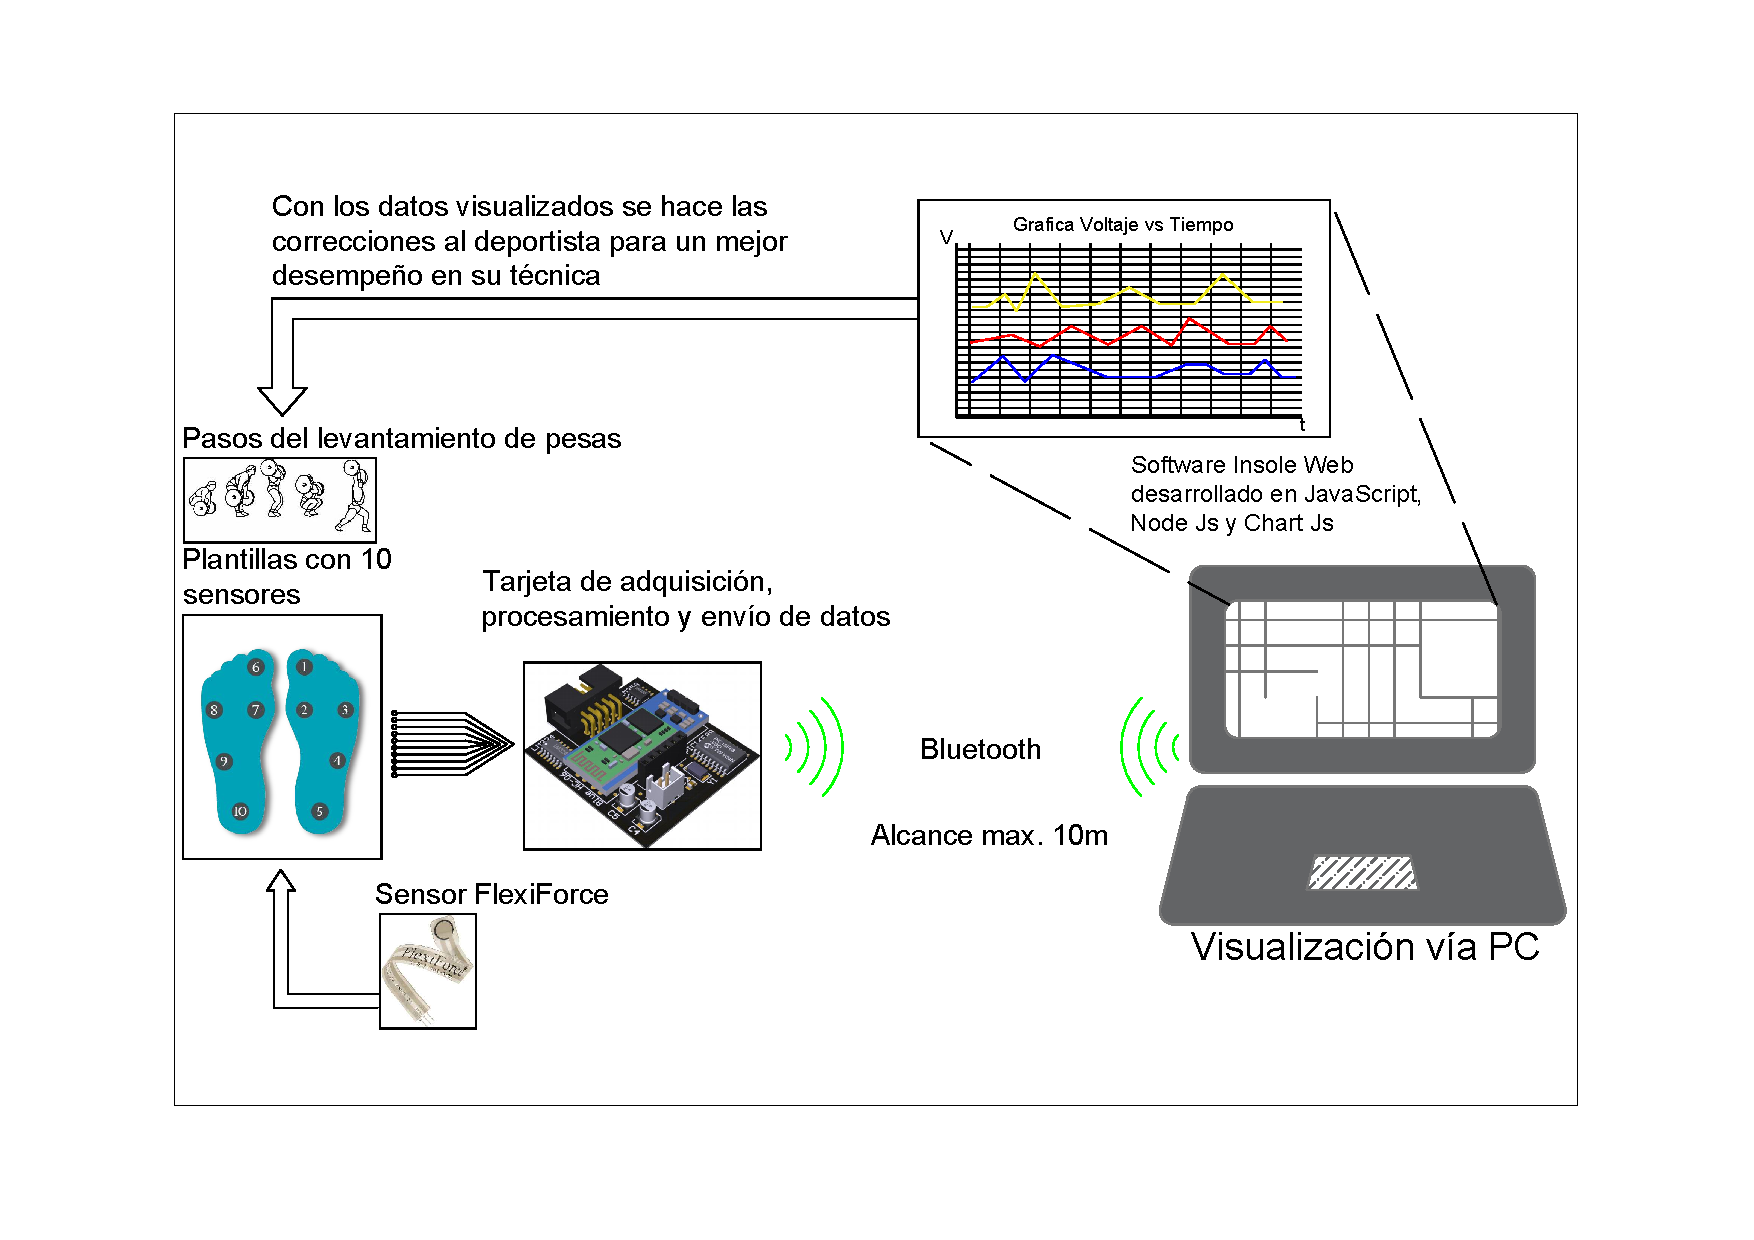
\includegraphics[width=1\textwidth]{./Documentos_PDF/Diagrama_de_Bloques_sistema_Insole.pdf}
\caption{Diagrama de Bloques del sistema de adquisición de datos.}
\label{fig:DiagramaBloque}
\end{figure*}

\newpage
\section{Código para el Microcontrolador PIC16F88}

\begin{lstlisting}[style=C]
///////////////////////////////////////////////////////////////////////////////////////////
//                                                                                       //
//                               PIC-Sensor_Plantilla1-UTB                               //
//                         @author: Ivan Dario Echeverry Mancera                         //
//                                                                                       //
///////////////////////////////////////////////////////////////////////////////////////////
//                                                                                       //
//              uControlador: PIC16F88                     Lenguaje: C                   //
//           Oscilacionde cristal (Xtal): 12MHz                                          //
//                                                                                       //
///////////////////////////////////////////////////////////////////////////////////////////

unsigned int Sensado1;
unsigned int Sensado2;
unsigned int Sensado3;
unsigned int Sensado4;
unsigned int Sensado5;

char texto1[20];
char texto2[20];
char texto3[20];
char texto4[20];
char texto5[20];

void main() 
{

	TrisA.b0=1;
    TrisA.b1=1; 
    TrisA.b2=1;
    TrisA.b3=1;
    TrisA.b4=1;
    Trisb.b2=1;//RX entrada
  	Trisb.b5=0;//TX salida
    
  	ADC_init();
  	UART1_init(9600);
    
  	Delay_ms(1000); 
}

while(1)
{

	Sensado1 = ADC_Read(0);
	wordtostr(Sensado1,texto1);
    
	Sensado2 = ADC_Read(1);
	wordtostr(Sensado2,texto2);
    
	Sensado3 = ADC_Read(2);
	wordtostr(Sensado3,texto3);
    
	Sensado4 = ADC_Read(3);
	wordtostr(Sensado4,texto4);
    
	Sensado5 = ADC_Read(4);
	wordtostr(Sensado5,texto5);

                           UART1_Write_Text(texto1);
                           UART1_Write_Text(" ");

                           UART1_Write_Text(texto2);
                           UART1_Write_Text(" ");

                           UART1_Write_Text(texto3);
                           UART1_Write_Text(" ");

                           UART1_Write_Text(texto4);
                           UART1_Write_Text(" ");

                           UART1_Write_Text(texto5);
                           UART1_Write(0x0A);

 Delay_ms(100);
}

\end{lstlisting}

\newpage
\section{Código HTML}

\begin{lstlisting}[style=HTML5]
<!DOCTYPE html>
<html>
  <head>
    <link rel="stylesheet" href="https://cdnjs.cloudflare.com/ajax/libs/font-awesome/4.7.0/css/font-awesome.min.css">
    <link href="https://fonts.googleapis.com/icon?family=Material+Icons" rel="stylesheet">
    <link rel="icon" type="image/png" href="icon.png" />
    <meta charset="utf-8">
    <title>Insole</title>
    
    <style>
  #parrafo {
    background-color:#585858;
    margin: 10px;
    padding: 20px;
    -webkit-box-shadow: 10px 20px 39px 6px rgba(0,0,0,0.75);
    -moz-box-shadow: 10px 20px 39px 6px rgba(0,0,0,0.75);
    box-shadow: 10px 20px 39px 6px rgba(0,0,0,0.75);
    border-radius: 20px 20px 20px 20px;
    -moz-border-radius: 20px 20px 20px 20px;
    -webkit-border-radius: 20px 20px 20px 20px;
    border: 0px solid #000000;
  }
  #izq {
    background-color:#FFFFFF;
    margin: 10px;
    padding: 0px;
    -webkit-box-shadow: 10px 20px 30px 6px rgba(0,0,0,0.75);
    -moz-box-shadow: 10px 20px 30px 6px rgba(0,0,0,0.75);
    box-shadow: 10px 20px 30px 6px rgba(0,0,0,0.75);
    border-radius: 20px 20px 20px 20px;
    -moz-border-radius: 20px 20px 20px 20px;
    -webkit-border-radius: 20px 20px 20px 20px;
    border: 0px solid #000000;
  }
  #titulo {
    background-color:#585858;
    margin: 20px;
    -webkit-box-shadow: 10px 20px 39px 6px rgba(0,0,0,0.75);
    -moz-box-shadow: 10px 20px 39px 6px rgba(0,0,0,0.75);
    box-shadow: 10px 20px 39px 6px rgba(0,0,0,0.75);
    border-radius: 20px 20px 20px 20px;
    -moz-border-radius: 20px 20px 20px 20px;
    -webkit-border-radius: 20px 20px 20px 20px;
    border: 0px solid #000000;
  }
  #iconos {
    display: block;
    margin: 0px;
    padding: 0px;
    border: 0px;
    font-size: 2em;
    -webkit-margin-before: 0.1em;
    -webkit-margin-after: 0.1em;
    -webkit-margin-start: 0px;
    -webkit-margin-end: 0px;
    font-weight: bold;
  }
  #titulografica {
    background-color:#585858;
    margin: 0px;
    padding: 20px;
    border-radius: 20px 20px 0px 0px;
    -moz-border-radius: 20px 20px 0px 0px;
    -webkit-border-radius: 20px 20px 0px 0px;
  }
  #Der {
    margin: 0px;
    padding: 150px 0px 0px 0px;
  }
  </style>
  
  </head>
  <body>
  
    <div id="titulo">
    <h1 align=center><font color="White">INSOLE</font></h1>
    </div>
    <h1 id="iconos" align="center"><i class="material-icons md-16">accessibility</i><i class="material-icons md-16">bluetooth_searching</i><i class="material-icons md-16">autorenew</i><i class="material-icons md-16">all_inclusive</i></h1>
    <div class="box">
      <div class="container">
        <div id="izq" style="float: left; width: 83%">
          <p id="titulografica"><font color="White">Grafica plantilla derecha - Insole</font></p>
          <canvas id="myCanvas" style="display: block; width:100%"></canvas>
        </div>
      </div>
      
        <script src="https://cdnjs.cloudflare.com/ajax/libs/Chart.js/2.7.2/Chart.min.js" charset="utf-8"></script>
        <script src="/socket.io/socket.io.js" charset="utf-8"></script>
        <script>
          var socket = io();
          var chartOptions = {
            scales: {
              xAxes: [{
                scaleLabel: {
                  display: true,
                  labelString: "Numero de Datos Obtenidos"
                }
              }],
              yAxes: [{
                ticks: {
                  min: 0.8,
                  max: 5,
                  stepSize: 0.1
                },
                scaleLabel: {
                  display: true,
                  labelString: "Voltaje [V]"
                }
              }]
            },
            responsive: false
          };
          
          var ctx = document.getElementById("myCanvas").getContext('2d');
          var myChart = new Chart(ctx, {
            type: 'line',
            data: {
              labels: [],
              datasets: [{
                label: "Sensor 1",
                fill: false,
                borderColor: 'rgb(16, 119, 251)',
                backgroundColor: 'rgb(16, 119, 251)',
                data: []
              },{
                label: "Sensor 2",
                fill: false,
                borderColor: "rgb(254, 189, 5)",
                backgroundColor: "rgb(254, 189, 5)",
                data: []
              }, {
                label: "Sensor 3",
                fill: false,
                borderColor: "rgb(77, 222, 5)",
                backgroundColor: "rgb(77, 222, 5)",
                data: []
              }, {
                label: "Sensor 4",
                fill: false,
                borderColor: "rgb(234, 49, 42)",
                backgroundColor: "rgb(234, 49, 42)",
                data: []
              }, {
                label: "Sensor 5",
                fill: false,
                borderColor: "rgb(218, 1, 218)",
                backgroundColor: "rgb(218, 1, 218)",
                data: []
              }]
            },
            options: chartOptions
          });
          
          var counter = 0;
          var DATA_LIMIT = 300;
          var labels = myChart.data.labels;
          socket.on('sen:data', function (senArray) {
            labels.push(counter++);
            var isFull = labels.length === DATA_LIMIT;
            if(isFull) labels.shift();
            senArray.forEach((sen, index) => {
              var chartData = myChart.data.datasets[index];
              chartData.data.push(sen);
              if(isFull) chartData.data.shift();
            });
            
            myChart.update();
          });
          </script>
          
        <div class="container">
          <div id="Der" style="float: right; width: 14%">
            <img src="plantilla.png" style="margin-left: auto; margin-right: auto; display: block; width: 70%;"/>
            <img src="utb.png" style="margin-left: auto; margin-right: auto; display: block; width: 80%; padding: 30px 0px 20px 0px;"/>
            <p id="designed" align="center" style="margin:0px; position: fixed;">&copy; 2018 - Designed by Ivan Echeverry</p>
          </div>
        </div>
    </div>
  </body>
</html>
\end{lstlisting}

\section{Código JavaScript}
\begin{lstlisting}[style=HTML5]
const path = require('path');
const http = require('http');
const express = require('express');
const socketIo = require('socket.io');

const app = express();
const server = http.createServer(app);
const io = socketIo.listen(server);

io.on('conection', function (socket) {
  console.log('a new socket connected');
});

app.use(express.static(path.join(__dirname, 'public')));

app.get('/', (req, res, next) => {
  res.sendFile(__dirname + '/index.html');
});

//SERIAL COMUNICATION
const SerialPort = require('serialport');
const Readline = SerialPort.parsers.Readline;
//const parser = new Readline();

const mySerial = new SerialPort('COM1', {
  baudRate: 9600
});

const parser = mySerial.pipe(new Readline({ delimeter: '\r\n'}));

parser.on('open', function () {
  console.log('Opened Serial Port');
});

parser.on('data', function (data) {
  console.log(data)
  //asumiendo que cada 1 recibe un datos siempre!
  const res = data
  .trim()
  .split("   ")
  .map(r => (r*5)/1023  );

  io.emit('sen:data', res);
});

mySerial.on('error', function (err){
  console.log(err);
});

server.listen(3000, () => {
  console.log('server on port ', 3000);
});
\end{lstlisting}

\newpage

\section{Esquemático del Circuito}

\begin{figure}[H]
\centering
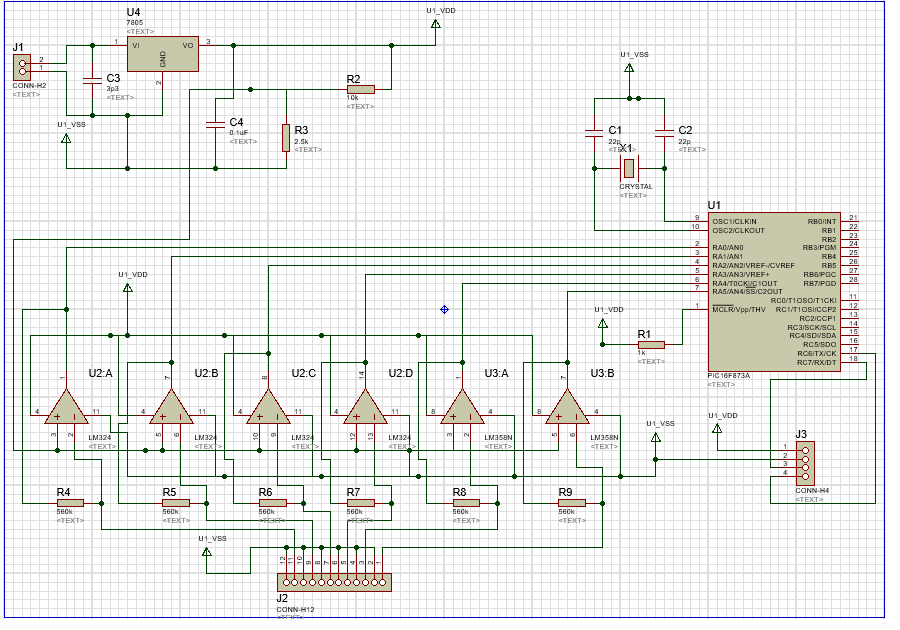
\includegraphics[width=1\textwidth]{./image/esquematico.png}
\caption{Esquemático}
\label{fig:esquematico}
\end{figure}

\newpage

\section{Documentación del Diseño PCB}

\begin{figure}[H]
\centering
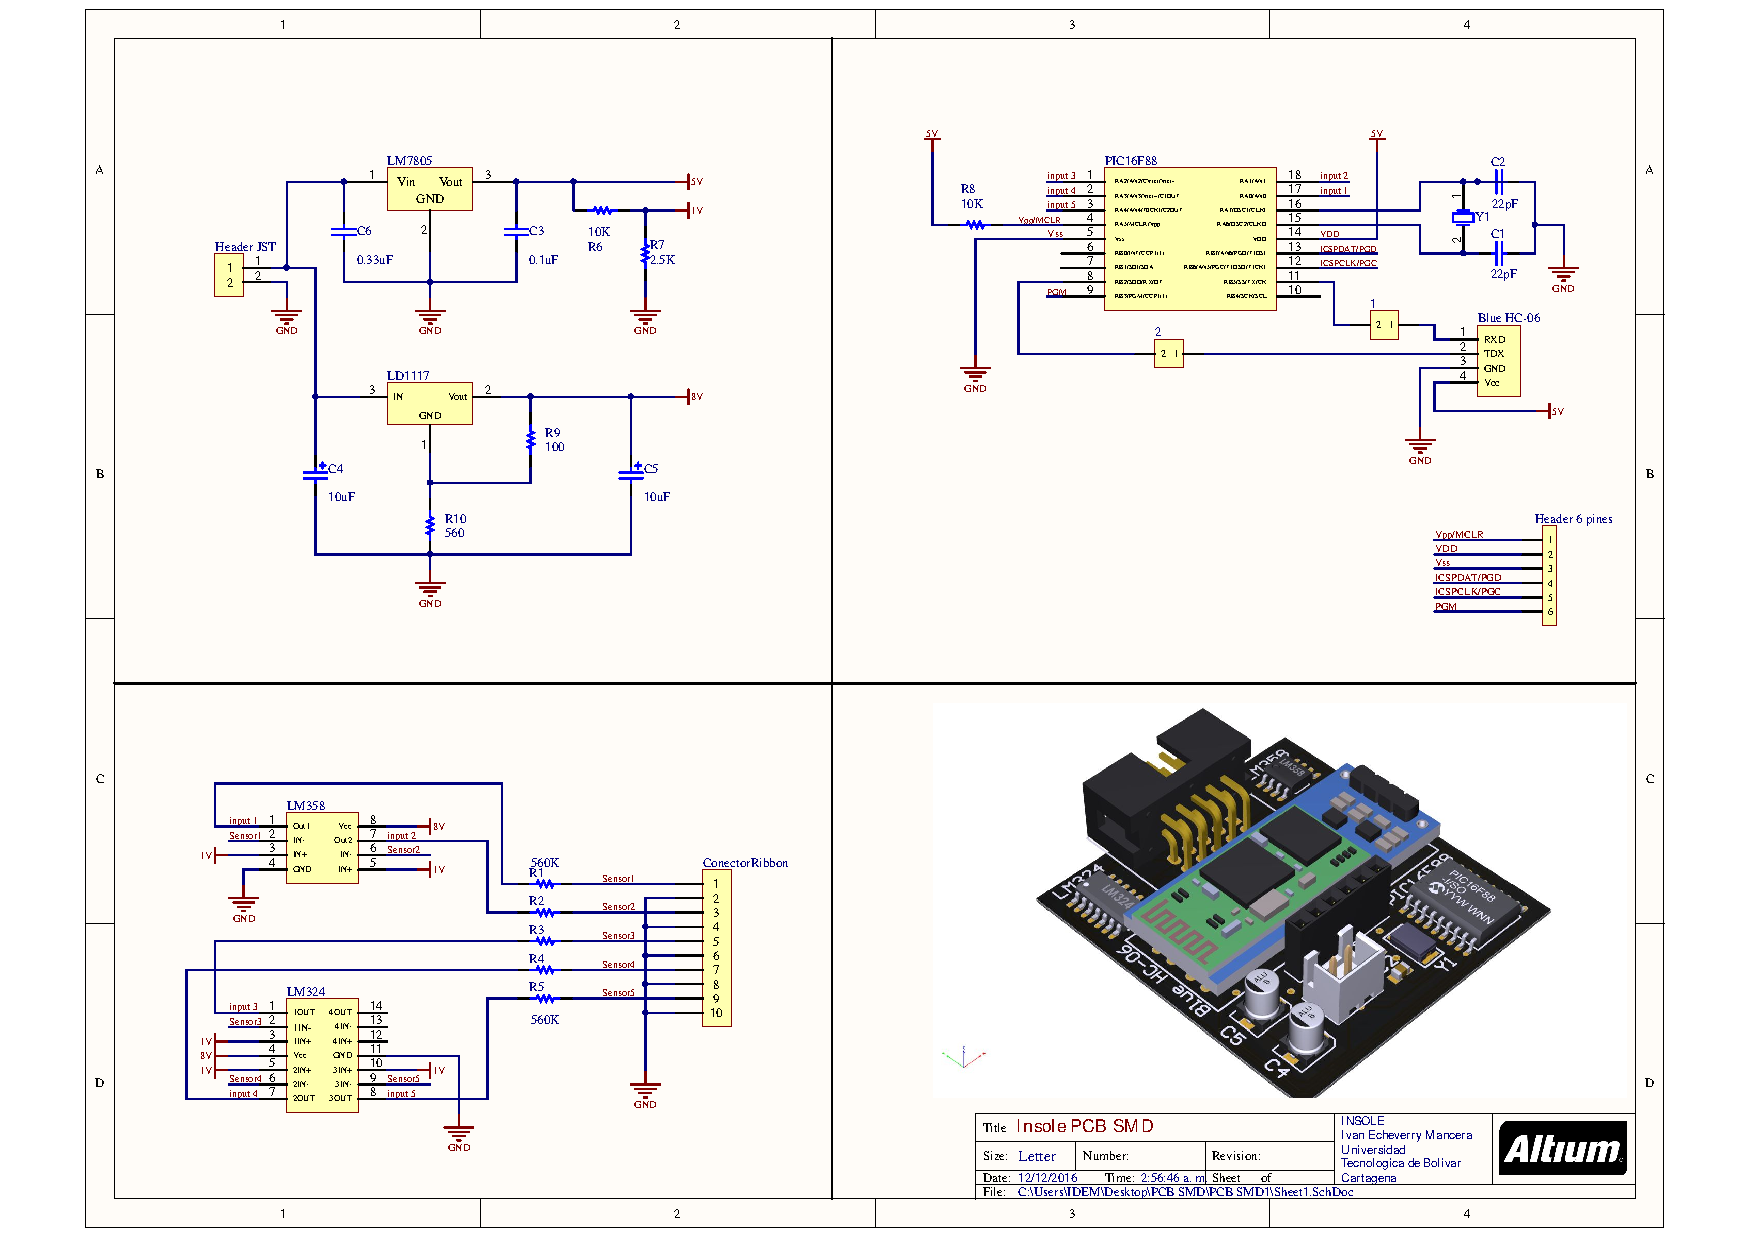
\includegraphics[width=1\textwidth]{./Documentos_PDF/DiagramaElectronico.pdf}
\caption{Diagrama Electrónico}
\label{fig:DiagramaElectronico}
\end{figure}

\begin{figure}[H]
\centering
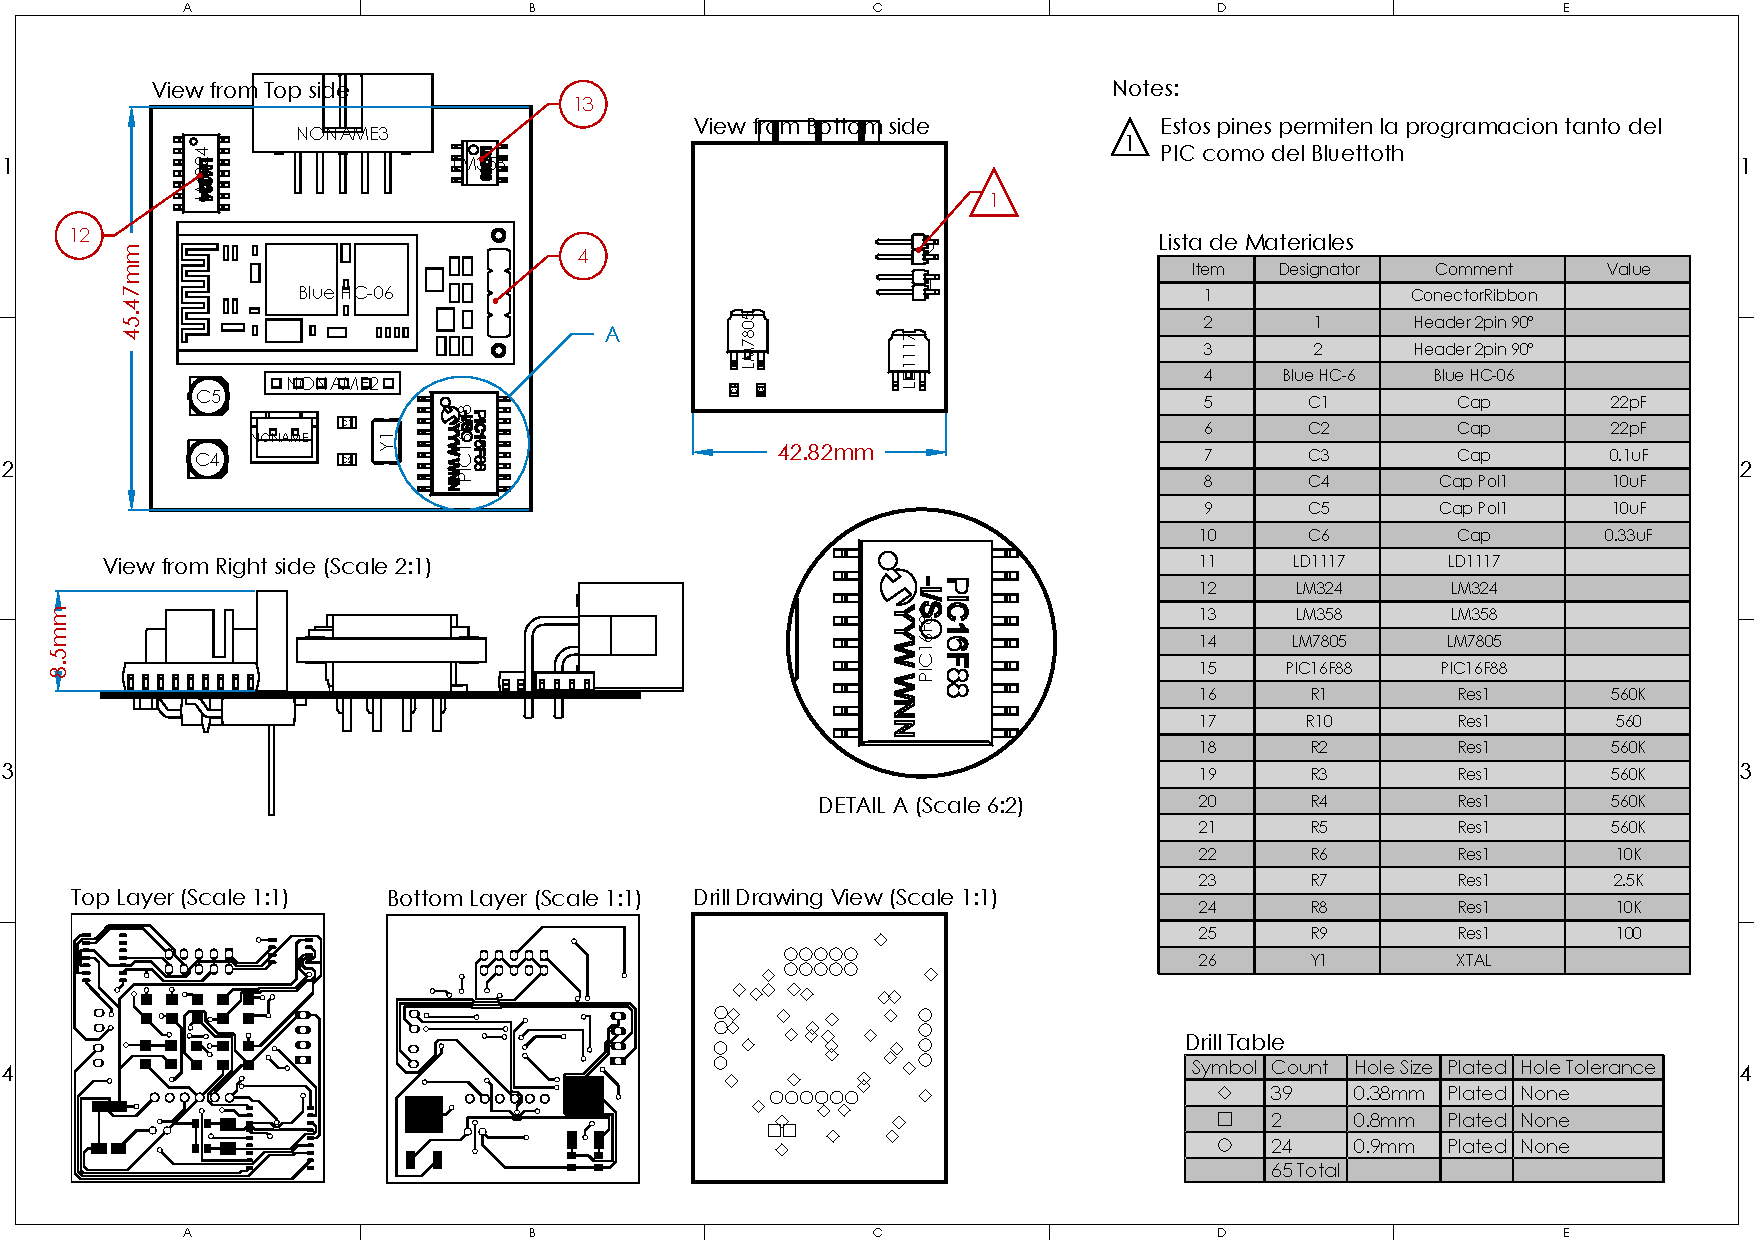
\includegraphics[width=1\textwidth]{./Documentos_PDF/Detalle_PCB.pdf}
\caption{Detalles del PCB}
\label{fig:PCB_Detalles}
\end{figure}

\begin{figure}[H]
\centering
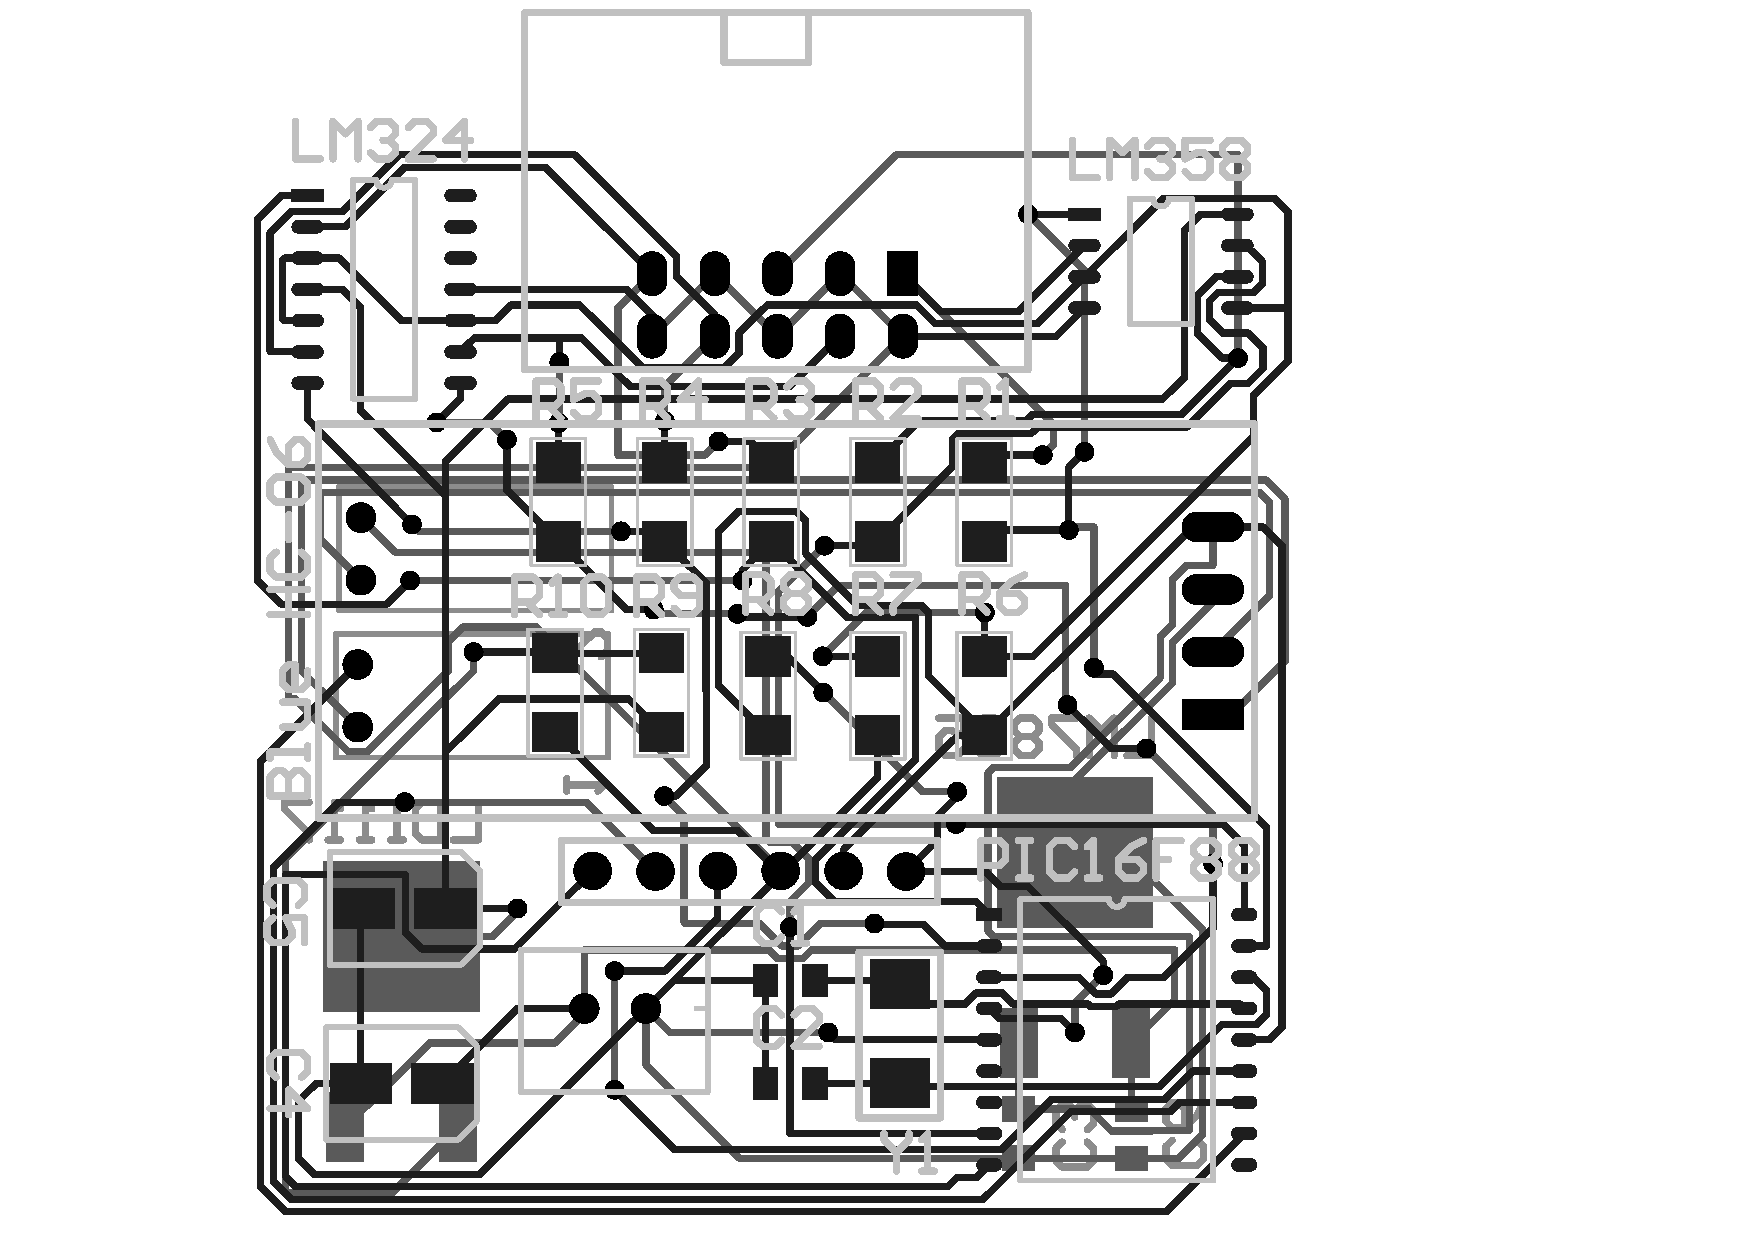
\includegraphics[width=1\textwidth]{./Documentos_PDF/Pistas_PCB.pdf}
\caption{Diseño de Pistas}
\label{fig:Pistas_PCB}
\end{figure}

\begin{figure}[H]
\centering
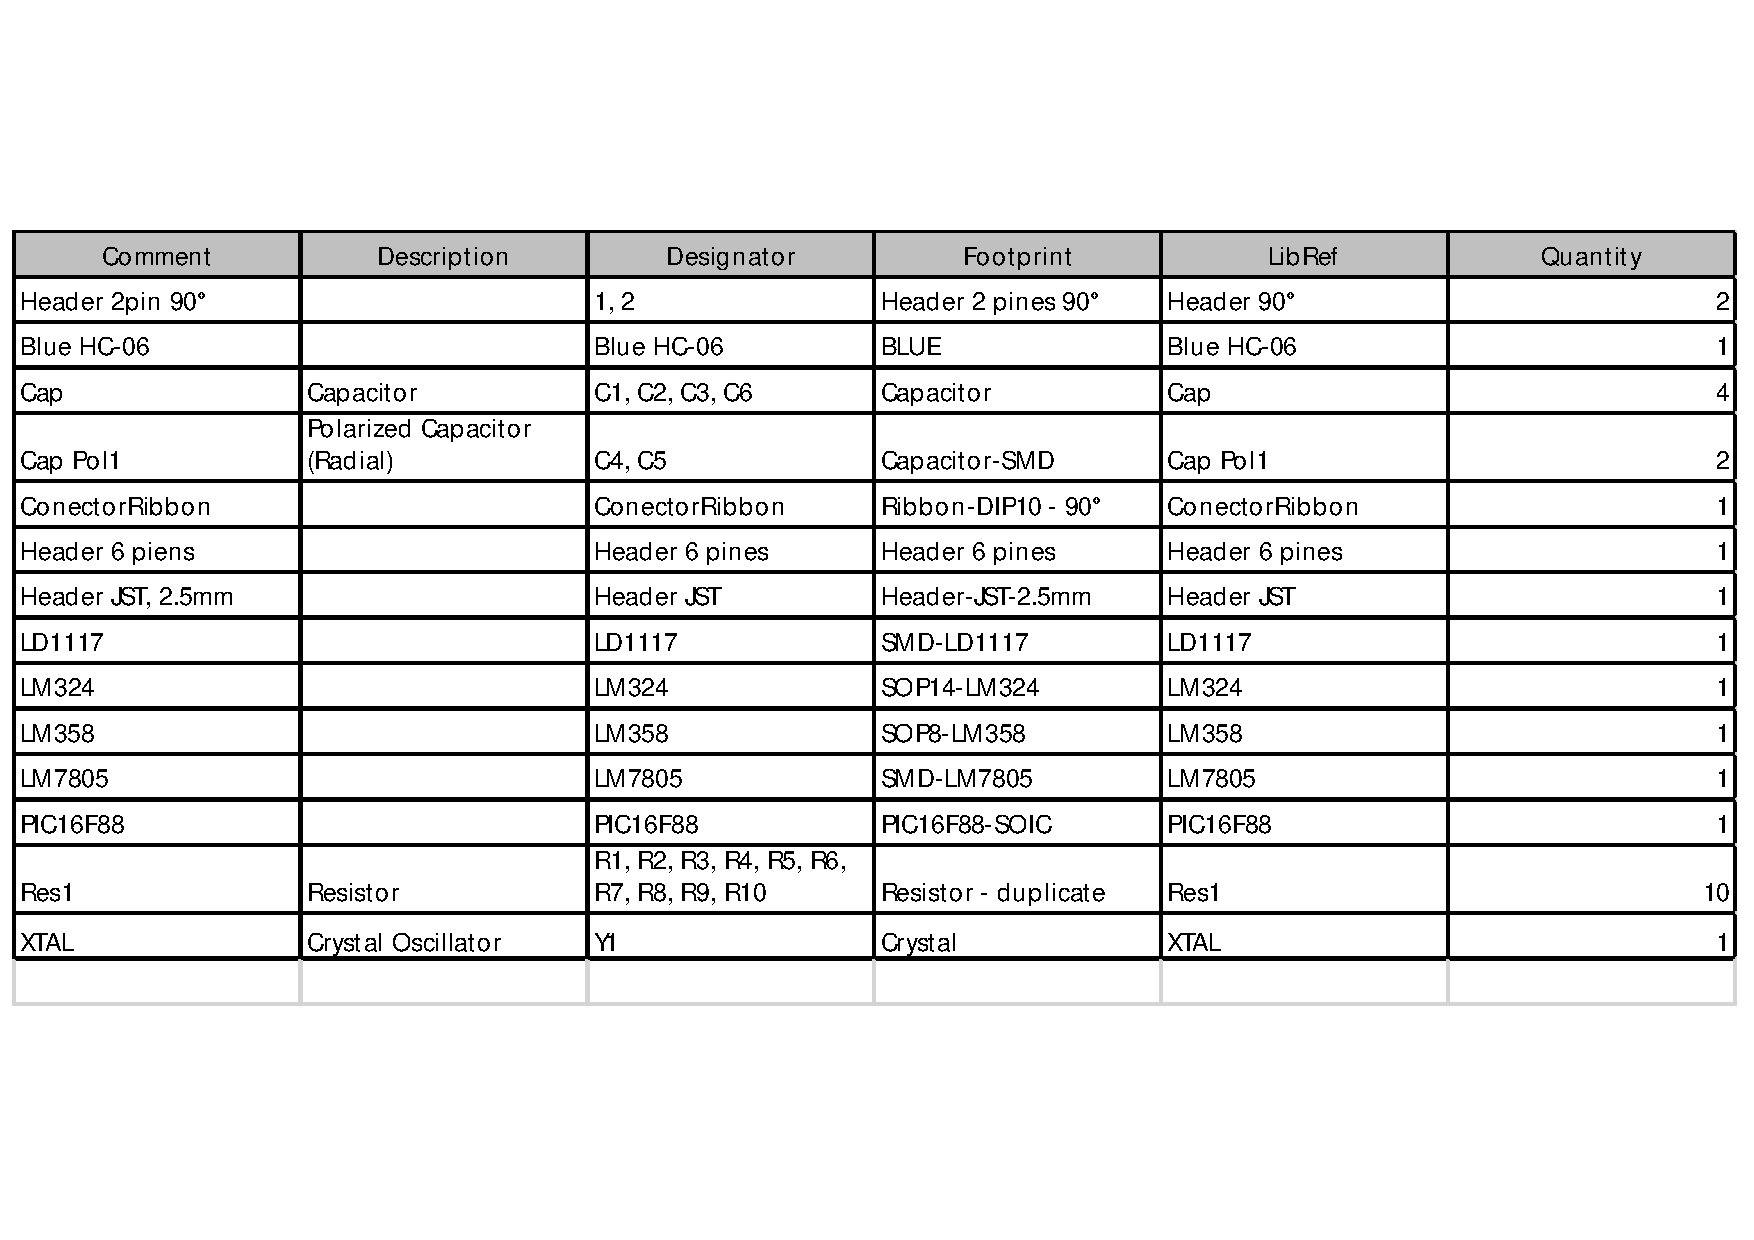
\includegraphics[width=1\textwidth]{./Documentos_PDF/Lista_Materiales.pdf}
\caption{Listas de Materiales PCB}
\label{fig:Lista_Materiales}
\end{figure}

\newpage

\section{Fotos del Sistema Insole}

\begin{figure}[H]
\centering
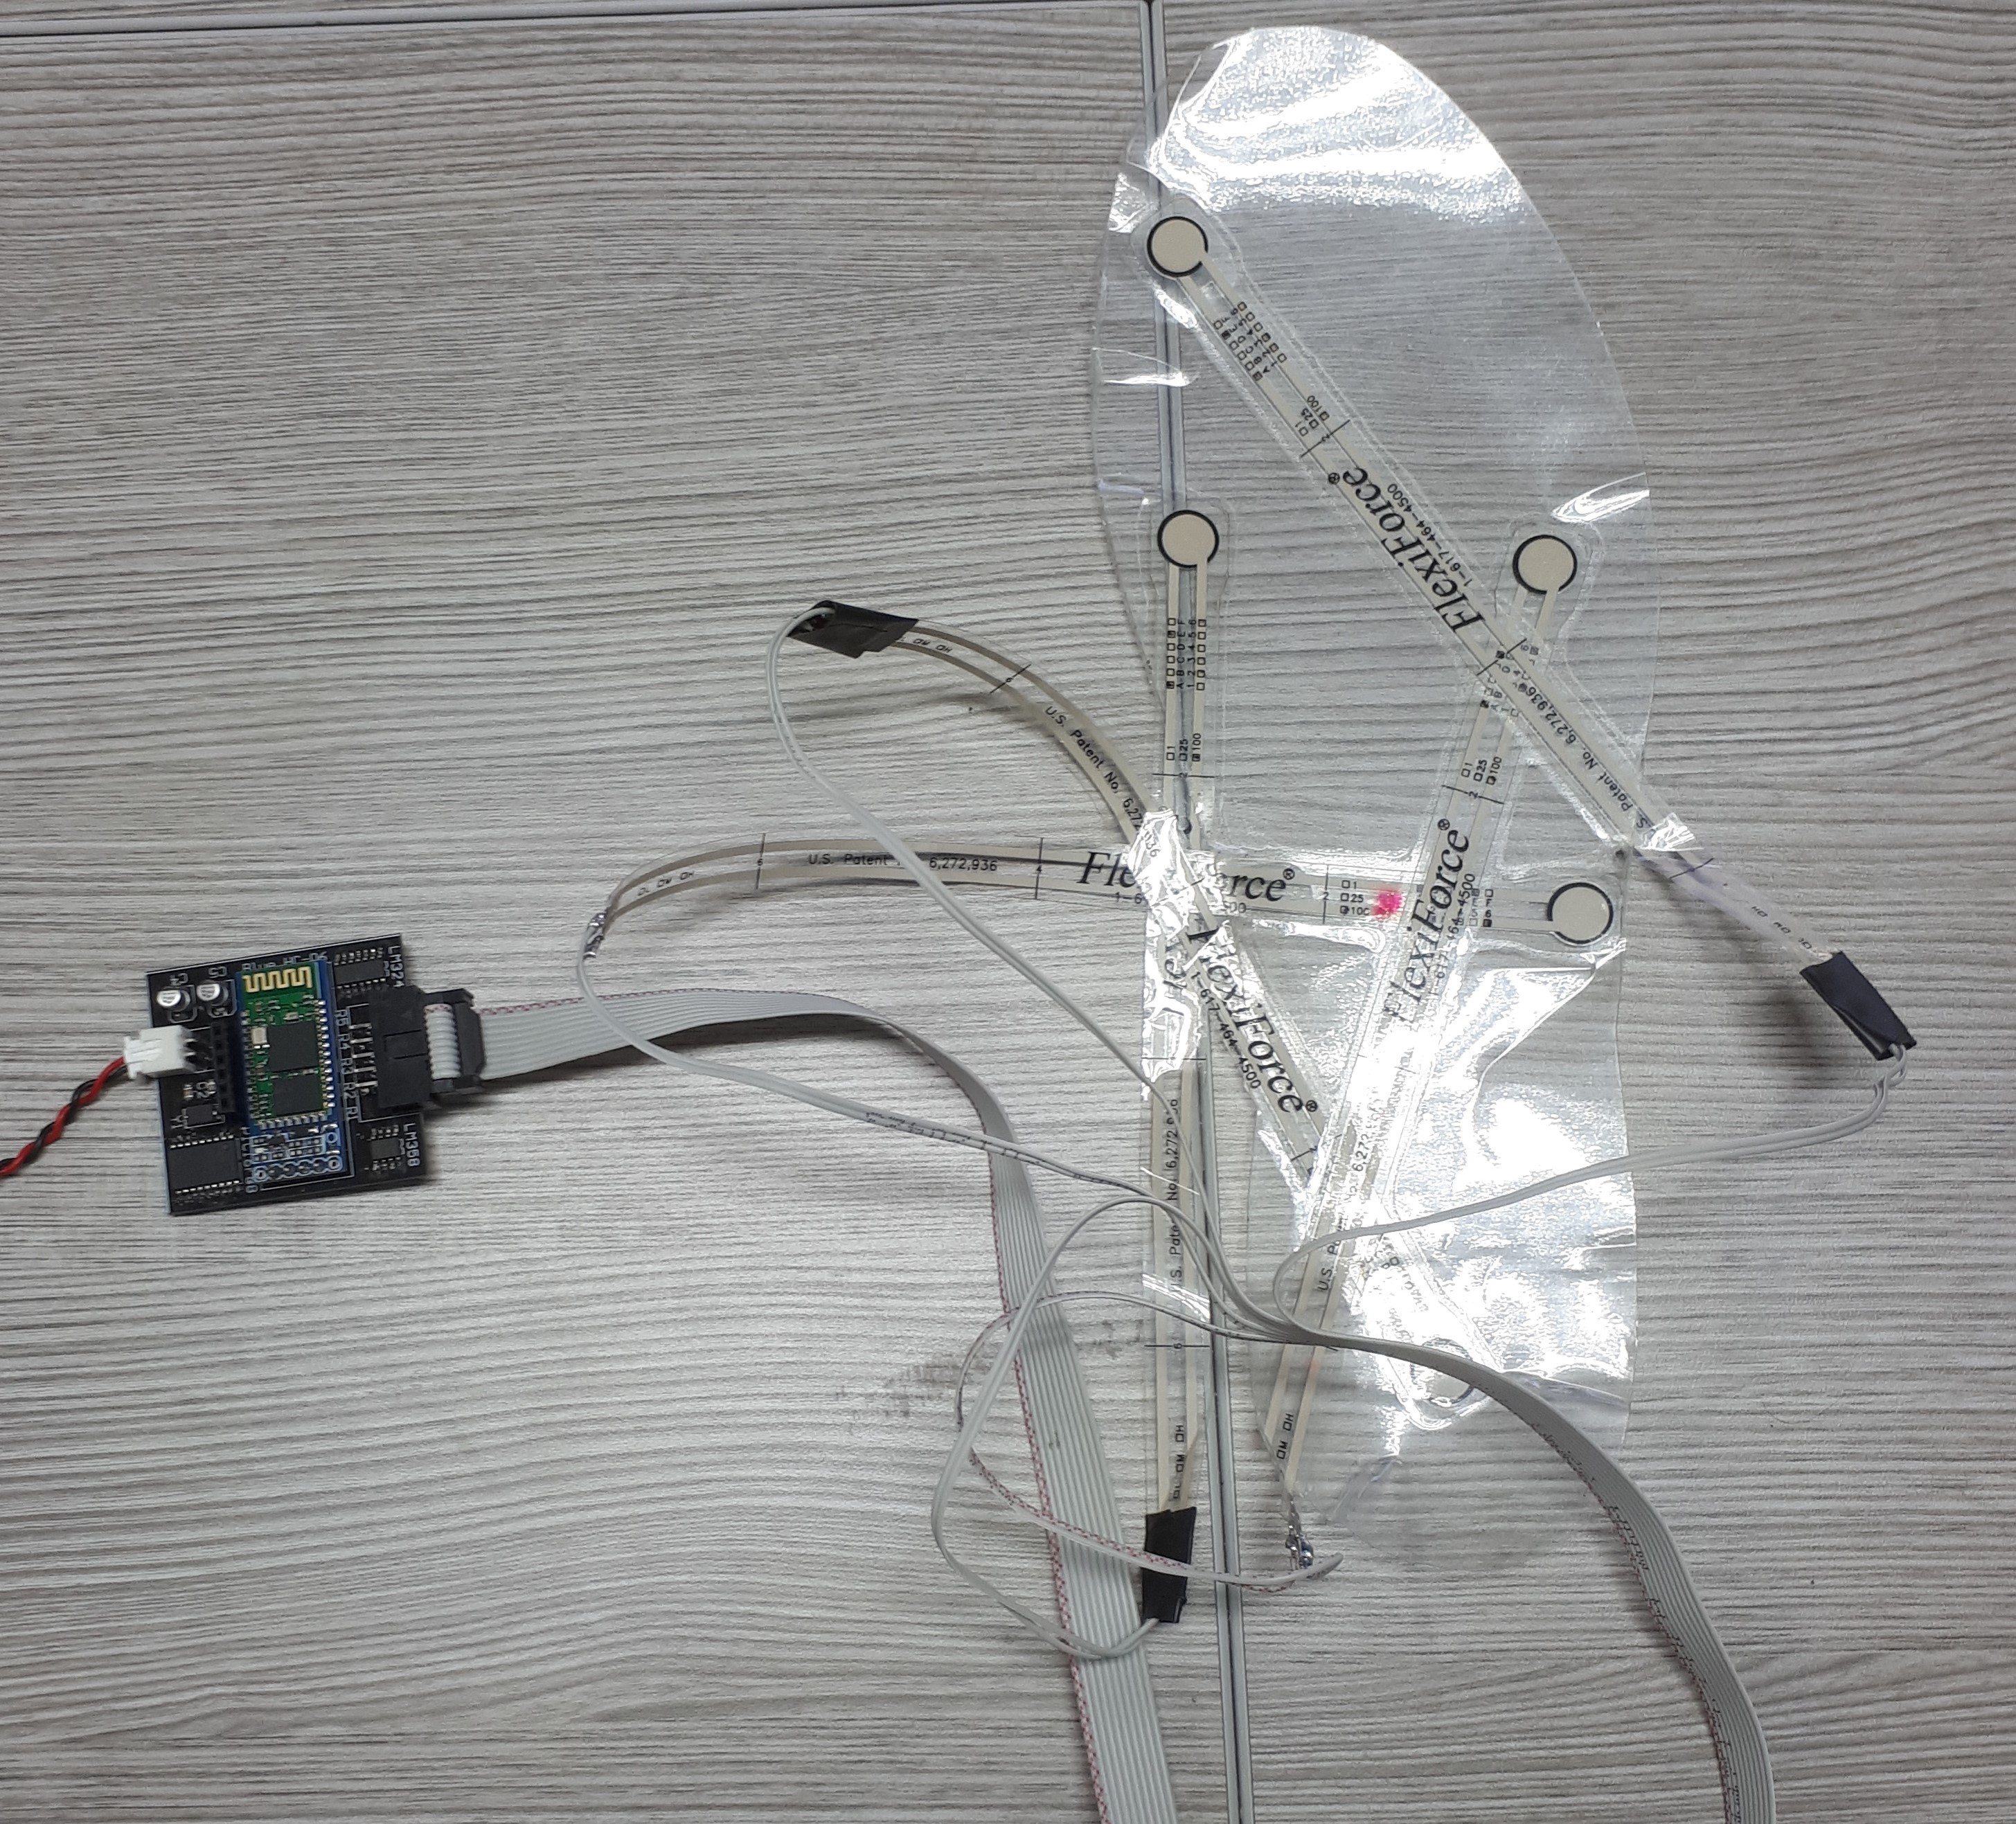
\includegraphics[width=1\textwidth]{./image/foto3.jpg}
\caption{Sistema de plantilla Insole Vista 1.}
\label{fig:plantillavista1}
\end{figure}

\begin{figure}[H]
\centering
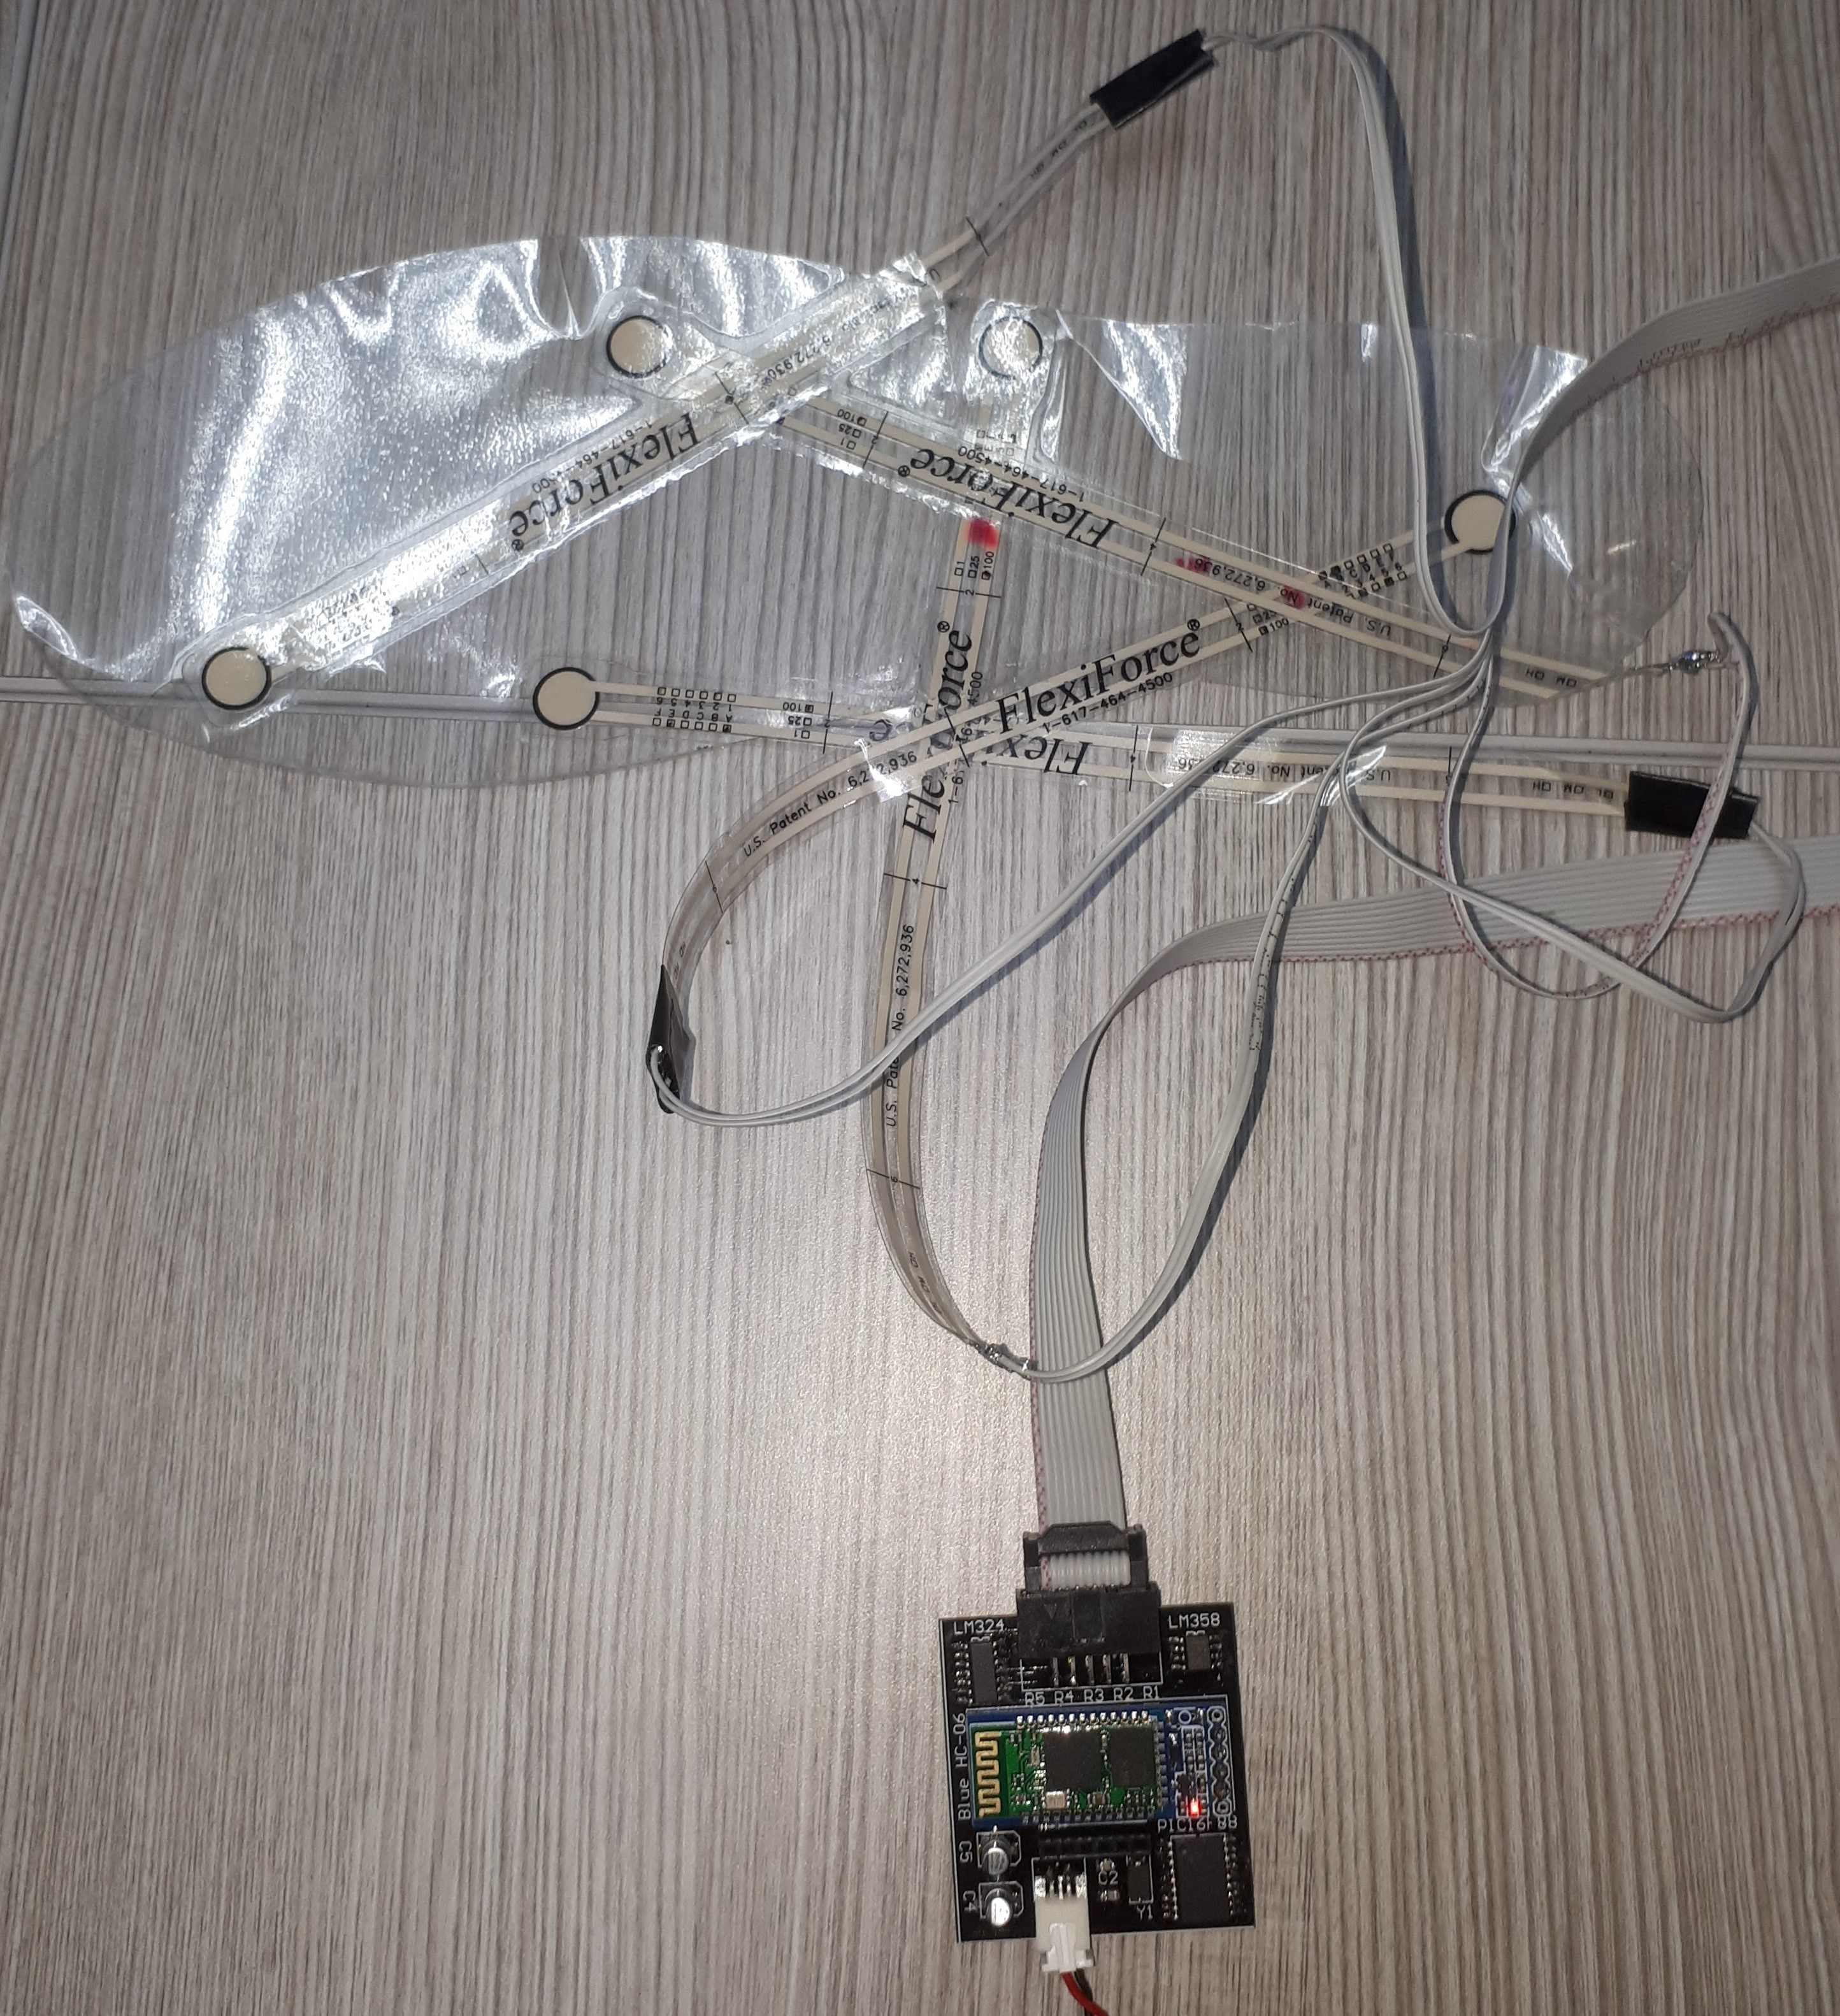
\includegraphics[width=1\textwidth]{./image/foto2.jpg}
\caption{Sistema de plantilla Insole Vista 2.}
\label{fig:plantillavista2}
\end{figure}

\begin{figure}[H]
\centering
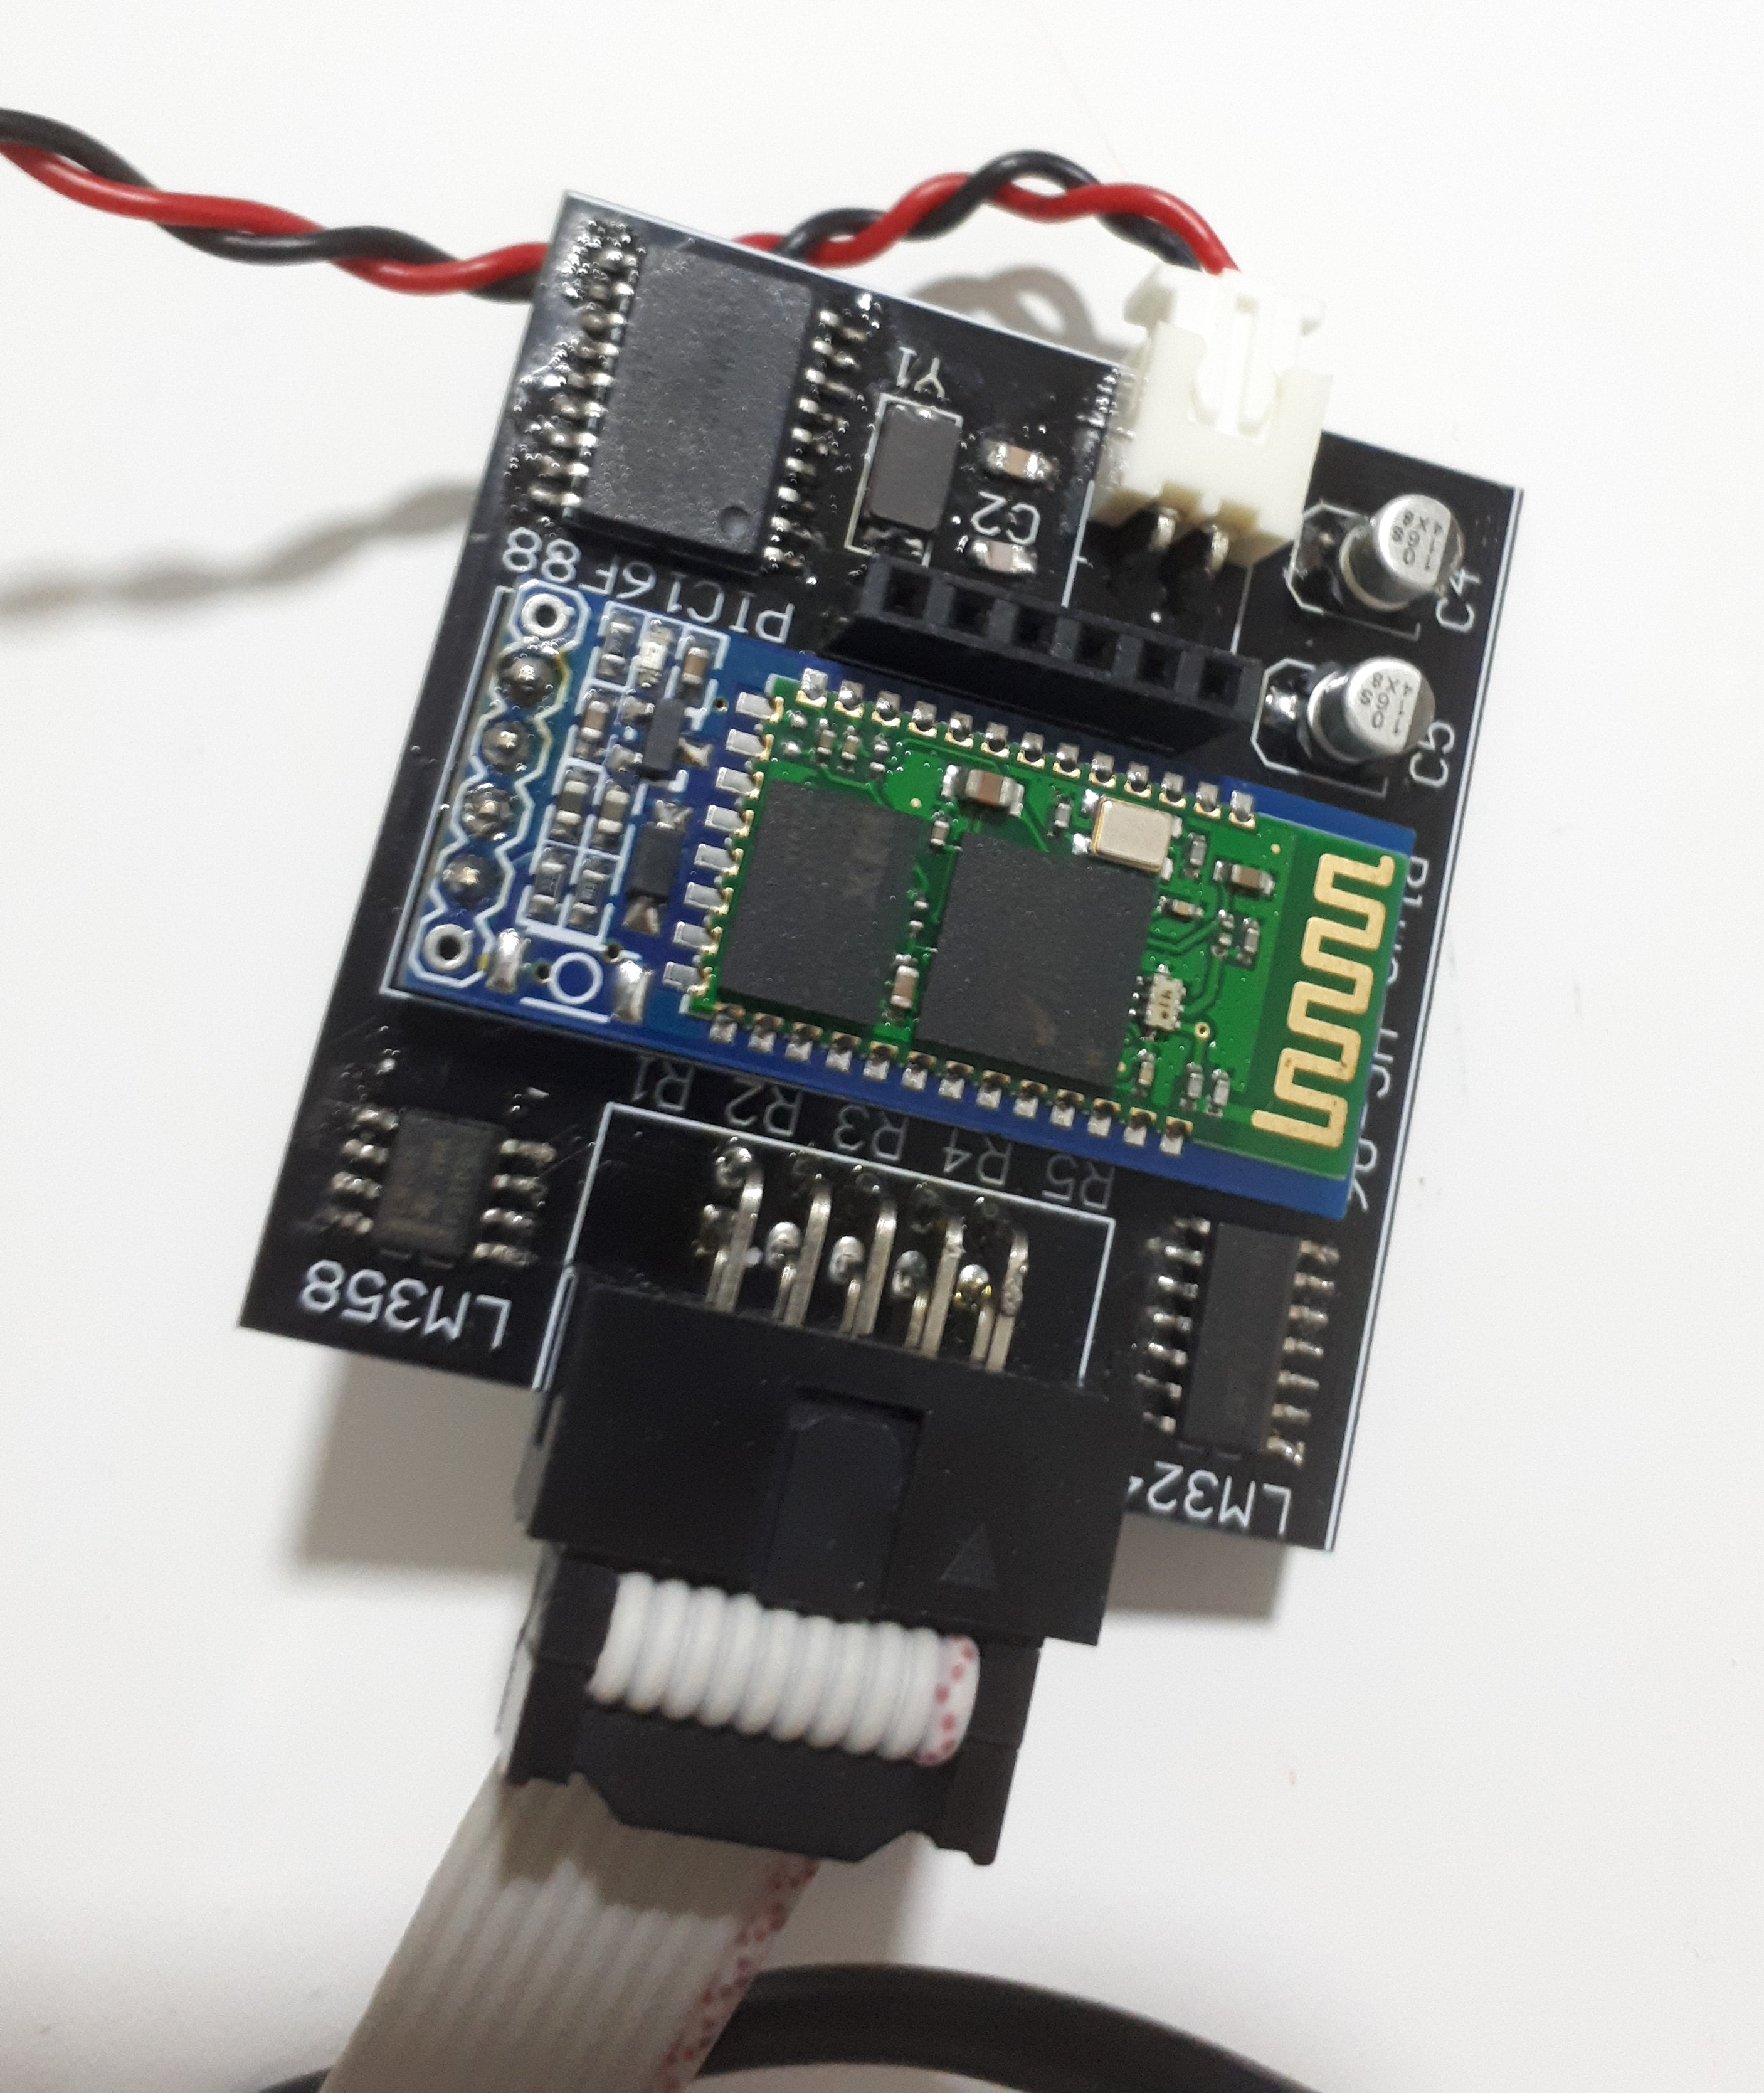
\includegraphics[width=1\textwidth]{./image/foto1.jpg}
\caption{Tarjeta electrónica captadora y transmisora de los datos.}
\label{fig:Tarjeta}
\end{figure}




